\chapter{Scenario}\label{ch:scenario}

\section{Communication}


The free space path loss (FSPL) is the loss in signal strength that occurs when an electromagnetic wave travels over a line of sight path in free space. In these circumstances there are no obstacles that might cause the signal to be reflected, refracted, or that might cause additional attenuation. Equation \ref{eq:path_losses} represents the loss in signal strength.

\begin{equation}\label{eq:path_losses}
L = 20log\left (\frac{4\pi d}{\lambda} \right)
\end{equation}

The wave length can also be described by a relationship between the frequency and the velocity which is the light speed because radio waves are electromagnetic waves. This relationship is described by the equation \ref{eq:vel_freq_wavelen1}.

\begin{equation}\label{eq:vel_freq_wavelen1}
\lambda = \frac{c}{f}
\end{equation}

Considering an area of a 

\begin{equation}\label{eq:vel_freq_wavelen2}
\lambda = \frac{c}{f} = \frac{3\times 10^{8}}{f\times 10^{6}}=\frac{300}{f}=\frac{3}{10f}
\end{equation}

\section{Rescue missions}
\subsection{What do they do today?}
\subsection{Compare the rescue missions}

\section{Pipeline survey}
The pipeline survey could be to transport oil from a factory to another facility. To ensure that there is no thiefs that want to steal the oil, they have to hire people to patrol. Instead they could use a drone to search the area.
\begin{figure}[hb]
  \centering
 % 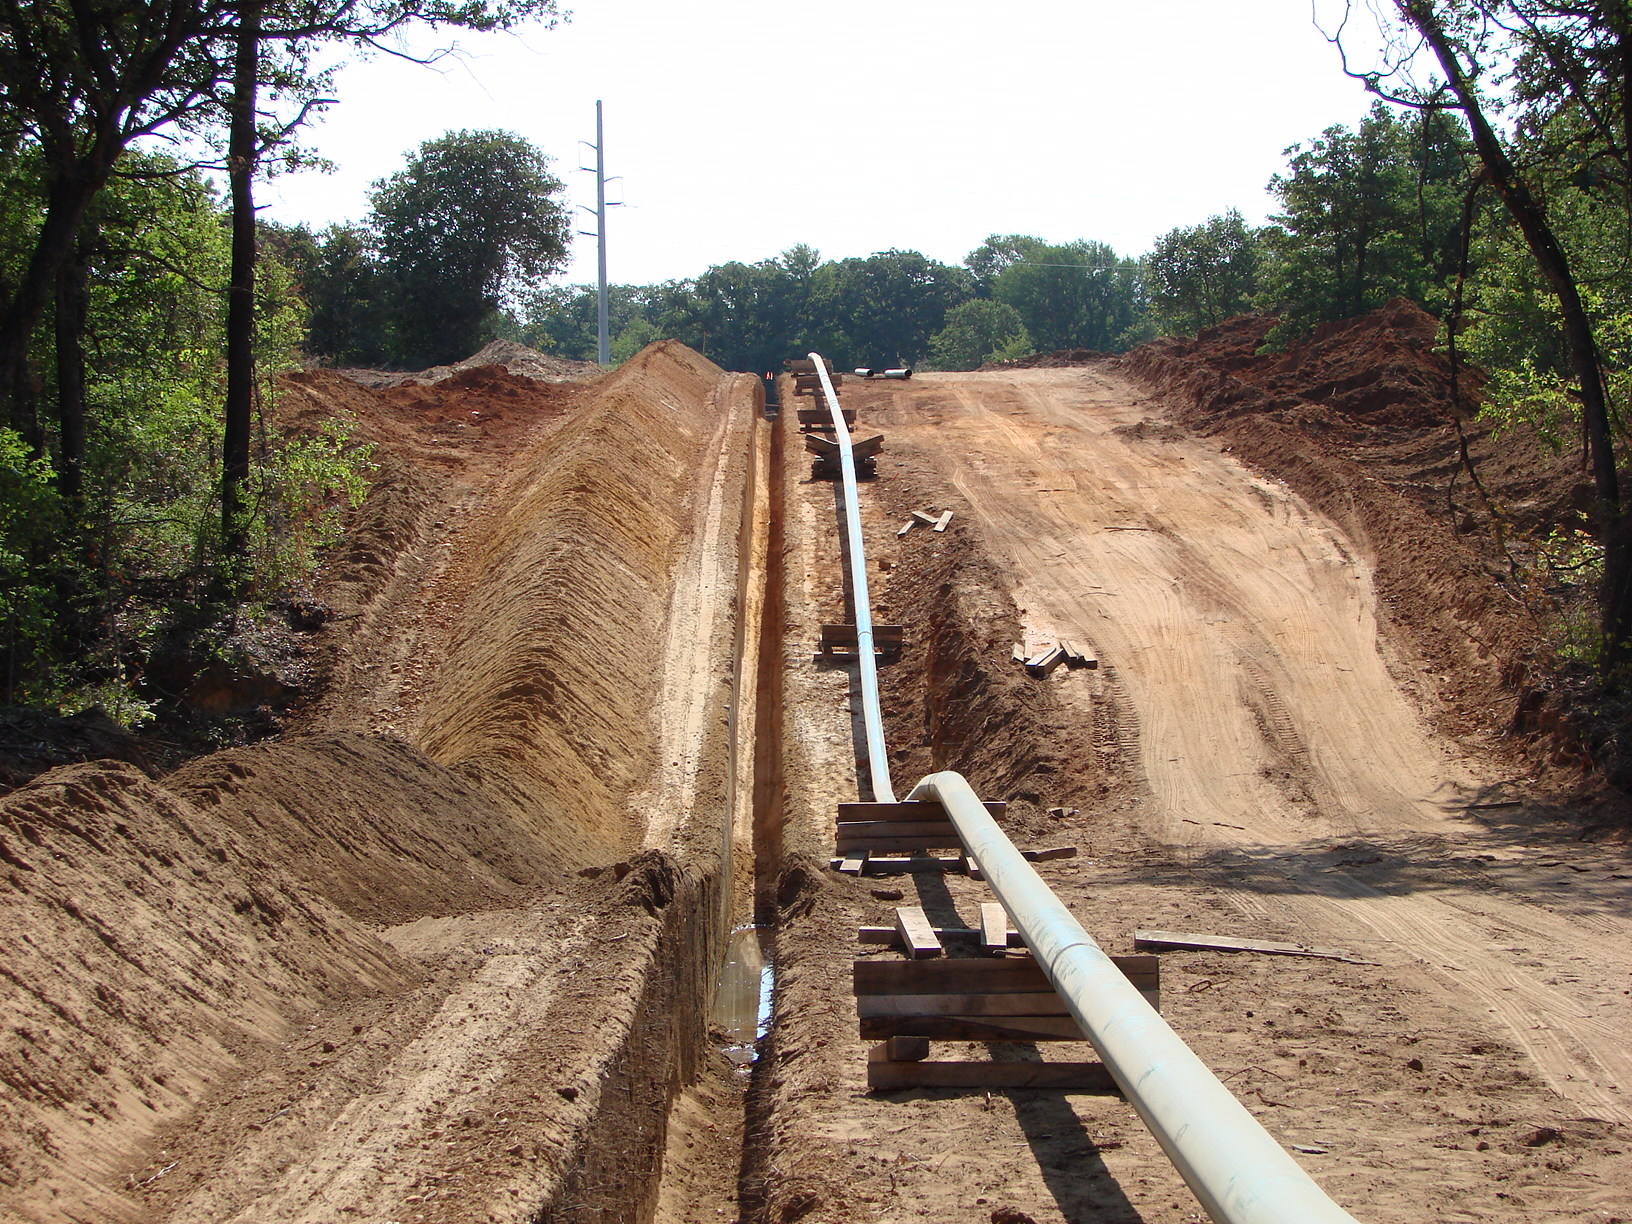
\includegraphics[width=3in]{figures/pipelinesurvey.png}
  \caption[Pipeline survey]
   {Pipeline survey}
\end{figure}
Potential danger
\begin{itemize}
\item Terrorist
\item Thiefs
\end{itemize}